\documentclass{article}
\usepackage[utf8]{inputenc}

\usepackage{sectsty}
\usepackage{fancyhdr}
\usepackage[top=1.25cm, bottom=2cm, left=2cm, right=2cm]{geometry}
\usepackage{tabularx,tabulary}
\usepackage{graphicx}

\title{Cahier des charges}
\begin{document}

%permet de souligner un certain type de partie
\sectionfont{\underline}

\maketitle
\section{Présentation du Projet}
	\subsection{Contexte et définition du problème}
		Le client souhaite faire effectuer des vols autonomes à un drone Bebop 2, avec un retour vidéo en temps réel sur un iPod Touch. Ce dernier pourra être placé dans un masque de vue à la première personne.\\
		La solution devra permettre à l'utilisateur de saisir un plan de vol sur une carte interactive et de le faire exécuter par le drone tout en ayant un retour vidéo sur l'iPod.\\
		\medbreak
        \begin{flushleft}
	        \textbf{Cas d'utilisation :} \\
	    \end{flushleft}
	    \begin{flushleft}
	    1) Un utilisateur souhaite effectuer une ronde avec un drone pour surveiller sa propriété au moindre effort.\\
	    Voici un exemple des étapes qu'il va suivre chronologiquement :\\
	     \end{flushleft}
	    \begin{center}
	    \renewcommand{\arraystretch}{2}
        \begin{tabularx}{15cm}{|c|X|}
            \hline
            1 & L'utilisateur lance l'application et arrive sur la page d'accueil.\\
            \hline
            2 & L'utilisateur lance la fonctionnalité de saisie du plan de vol sur une machine connectée au réseau local.\\
            \hline
            3 & L'utilisateur saisit le plan de vol sur la carte en spécifiant les points de passage du drone ainsi que les altitudes que le drone doit adopter au cours du vol. \\
            \hline
            4 & L'utilisateur valide la saisie de son plan de vol, ce dernier est enregistré. \\
            \hline
            5 & L'utilisateur allume le drone et y connecte sa machine en wifi. \\
            \hline
            6 & L'utilisateur lance la fonctionnalité d'exécution du plan de vol. \\
            \hline
            7 &  L'utilisateur démarre l'iPod touch, le connecte au réseau local et lance l'application de réception vidéo. La réception vidéo en temps réel sur l'iPod commence.\\
            \hline
            8 & L'utilisateur sélectionne parmi les plans de vols présents sur le drone celui qu'il vient de réaliser. \\
            \hline
            9 & L'utilisateur place l'iPod dans le masque FPV, le met sur sa tête, puis lance l'exécution du plan de vol. Le drone décolle. \\
            \hline
            10 & Le drone effectue le plan de vol choisi, l'utilisateur voit en temps réel ce que le drone filme. \\
            \hline
            11 & L'utilisateur souhaite stopper l'exécution de plan de vol : par exemple, il a repéré quelque chose d'anormal sur la zone de vol et souhaite s'y rendre au plus vite. Il active alors la procédure d'arrêt d'urgence sur sa machine et retire le masque FPV. Le drone stoppe l'exécution du plan de vol et attérit sur place si les conditions le permettent. \\
            \hline
        \end{tabularx}
        \end{center}
        
        \newpage
         \begin{flushleft}
        2) En hiver, un utilisateur souhaite faire effectuer au drone le tour de son jardin pour contrôler le niveau d'enneigement de celui-ci sans risquer de glisser.\\
        Voici un exemple des étapes qu'il va suivre chronologiquement : \\
         \end{flushleft}
	    \begin{center}
	    \renewcommand{\arraystretch}{2}
        \begin{tabularx}{15cm}{|c|X|}
            \hline
            1 & L'utilisateur lance l'application et arrive sur la page d'accueil.\\
            \hline
            2 & L'utilisateur lance la fonctionnalité de saisie du plan de vol sur une machine connectée au réseau local.\\
            \hline
            3 & L'utilisateur saisit le plan de vol sur la carte en spécifiant les points de passage du drone tout autour de son jardin et spécifie une altitude de quelques mètres. Le tracé est fait de manière à faire revenir le drone à son point de départ après avoir fait le tour du jardin. \\
            \hline
            4 & L'utilisateur valide la saisie de son plan de vol, ce dernier est enregistré. \\
            \hline
            5 & L'utilisateur allume le drone et y connecte sa machine en wifi. \\
            \hline
            6 & L'utilisateur lance la fonctionnalité d'exécution du plan de vol. \\
            \hline
            7 &  L'utilisateur démarre l'iPod touch, le connecte au réseau local et lance l'application de réception vidéo. La réception vidéo en temps réel sur l'iPod commence.\\
            \hline
            8 & L'utilisateur sélectionne parmi les plans de vols présents sur le drone celui qu'il vient de réaliser. \\
            \hline
            9 & L'utilisateur place l'iPod dans le masque FPV, le met sur sa tête, puis lance l'exécution du plan de vol. Le drone décolle. \\
            \hline
            10 & Le drone effectue le plan de vol choisi, l'utilisateur voit en temps réel ce que le drone filme et peut constater l'état d'enneigement de son jardin. \\
            \hline
            11 & L'utilisateur attend la fin de l'exécution du plan de vol pour retirer le masque et aller récupérer le drone une fois qu'il aura atterri à son point de départ, comme prévu.\\
            \hline
        \end{tabularx}
        \end{center}
        
	\subsection{Objectifs}
		\begin{enumerate}
        \item Permettre à l'utilisateur de saisir un plan de vol étape par étape sur une carte interactive et de spécifier les altitudes du drone à chaque point de passage.
        \item Permettre à l'utilisateur de sauvegarder son plan de vol pour le réutiliser plus tard.
		 \item Permettre à l'utilisateur de lancer l'exécution du plan de vol réalisé au préalable.
		 \item Rediriger le flux vidéo du drone vers l'iPod touch. 
		 \item Minimiser les latences vidéo (de l'ordre de la seconde).
		 \item Permettre d'arrêter le vol en cours en cas d'urgence.
		\end{enumerate}
\section{Expression des besoins}
	\subsection{Besoins fonctionnels}
	    \begin{center}
        \begin{tabularx}{15cm}{|c|p{4cm}|X|}
            \hline
            1 & Saisie du plan de vol & L'utilisateur doit pouvoir saisir un plan de vol sur une carte à travers une interface intuitive. L'utilisateur doit pouvoir spécifier l'altitude du drone à chaque waypoint (point de passage).\\
            \hline
            2 & Traduction du plan de vol au format Mavlink & Le plan de vol saisi graphiquement par l'utilisateur doit être converti au format Mavlink pour être ensuite envoyé au drone.\\
            \hline
            3 & Envoi du plan de vol au drone & La solution doit prendre en charge la récupération du plan de vol réalisé au préalable et son envoi au drone. \\
            \hline
            4 & Choix du plan de vol  & L'utilisateur doit pouvoir choisir le plan de vol enregistré sur le drone qu'il souhaite exécuter. \\
            \hline
            5 & Exécution du plan de vol  & Une fois le plan de vol choisi, l'utilisateur doit pouvoir en lancer l'exécution. \\
            \hline
            6 & Retour vidéo  & Tout au long du vol du drone, le retour vidéo de ce dernier doit être envoyé sur un iPod touch en temps réel et avec une latence minimale. \\
            \hline
            7 & Arrêt d'urgence  & A tout moment lors du vol, l'utilisateur doit pouvoir déclencher un arrêt d'urgence pour stopper l'exécution du plan de vol et faire atterrir le drone. \\
            \hline
        \end{tabularx}
        \end{center}
	\subsection{Besoins non fonctionnels}
	(à compléter)\\
\section{Solutions étudiées}
	\subsection{Comparatif des solutions}
	  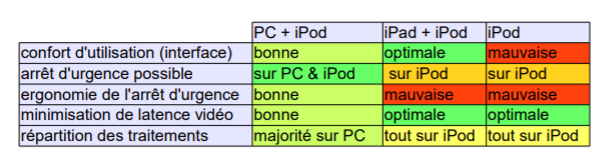
\includegraphics{comparatif.PNG}\\
	  Les architectures étudiées sont les suivantes, de gauche à droite dans le tableau : 
	  \begin{enumerate}
        \item une architecture utilisant un PC sous linux pour la saisie du plan de vol et qui commande le drone, ainsi qu'un iPod Touch sur lequel on redirige le flux vidéo.
        \item une architecture utilisant un iPad pour la saisie du plan de vol, ainsi qu'un iPod Touch qui commande le drone et récupère le flux vidéo.
         \item une architecture utilisant un iPod Touch pour la saisie du plan de vol, qui commande le drone et récupère le flux vidéo.
        \end{enumerate}
        Comme on peut le constater, la solution utilisant le PC et l'iPod Touch est plus avantageuse.\\
        C'est donc cette solution qui sera préférée.
\section{Contraintes}
	\subsection{Matériel}
		\begin{flushleft}
	        \textbf{Pour réaliser ce projet nous disposons du matériel suivant :}
	    \end{flushleft}
		\begin{enumerate}
        \item un drone Bebop 2;
        \item un iPod Touch (préciser version);
        \item un accès aux salles machines SAR équipées de machines sous OSX.
        \item un accès aux salles informatiques équipées de machines sous Linux.
        \end{enumerate}
        \begin{flushleft}
	        \textbf{Les contraintes techniques se la solution préférée sont :}
	    \end{flushleft}
		\begin{enumerate}
        \item Le PC sous Linux doit avoir deux cartes réseau : une pour pouvoir se connecter au drone en wifi, l'autre pour se connecter au réseau local pour rediriger le flux vidéo.
        \item Il faut un réseau local sur lequel sont connectés le PC et l'iPod Touch.
        \item Le réseau local doit avoir un accès internet.
        \end{enumerate}
	\subsection{Délais}
		Date de livraison du produit.\\
		Autres Échéances du projet par exemple le rendu du cahier des charges le .
		Contrainte de temps : contrainte la plus importante.\\
		(Lister les contraintes par ordre d'importance)
	\subsection{Autres contraintes}
	    \begin{flushleft}
	        \textbf{Concernant le plan de vol :} 
	    \end{flushleft}
	    \begin{enumerate}
            \item  L'application de saisie du plan de vol doit intégrer une carte interactive permettant de tracer ce dernier.
    		 \item On devra pouvoir spécifier l'altitude à laquelle le drone doit se trouver aux différents points du parcours.
		 \end{enumerate}
		
	    \begin{flushleft}
	        \textbf{Concernant le retour vidéo :}
	    \end{flushleft}
	     \begin{enumerate}
	     \item La qualité du retour vidéo est directement liée à la distance avec le serveur central (le PC) ainsi qu'à l'encombrement de l'espace dans lequel le drone vol. Un terrain avec des obstacles comme des bâtiments ou des arbres réduit fortement la porté du signal vidéo.
	     \item Le retour vidéo du drone doit être envoyé à un iPod Touch en temps réel.
	     \item Sa qualité doit être convenable (HD).
		 \item La latence du retour vidéo sur l'iPod doit être minimale (de l'ordre de la seconde), et la vidéo doit être fluide.
		 \end{enumerate}
		 
\section{Cinématique des écrans :}

 \begin{enumerate}
 \item Lors de l'ouverture de la page, la carte est vierge:\\
 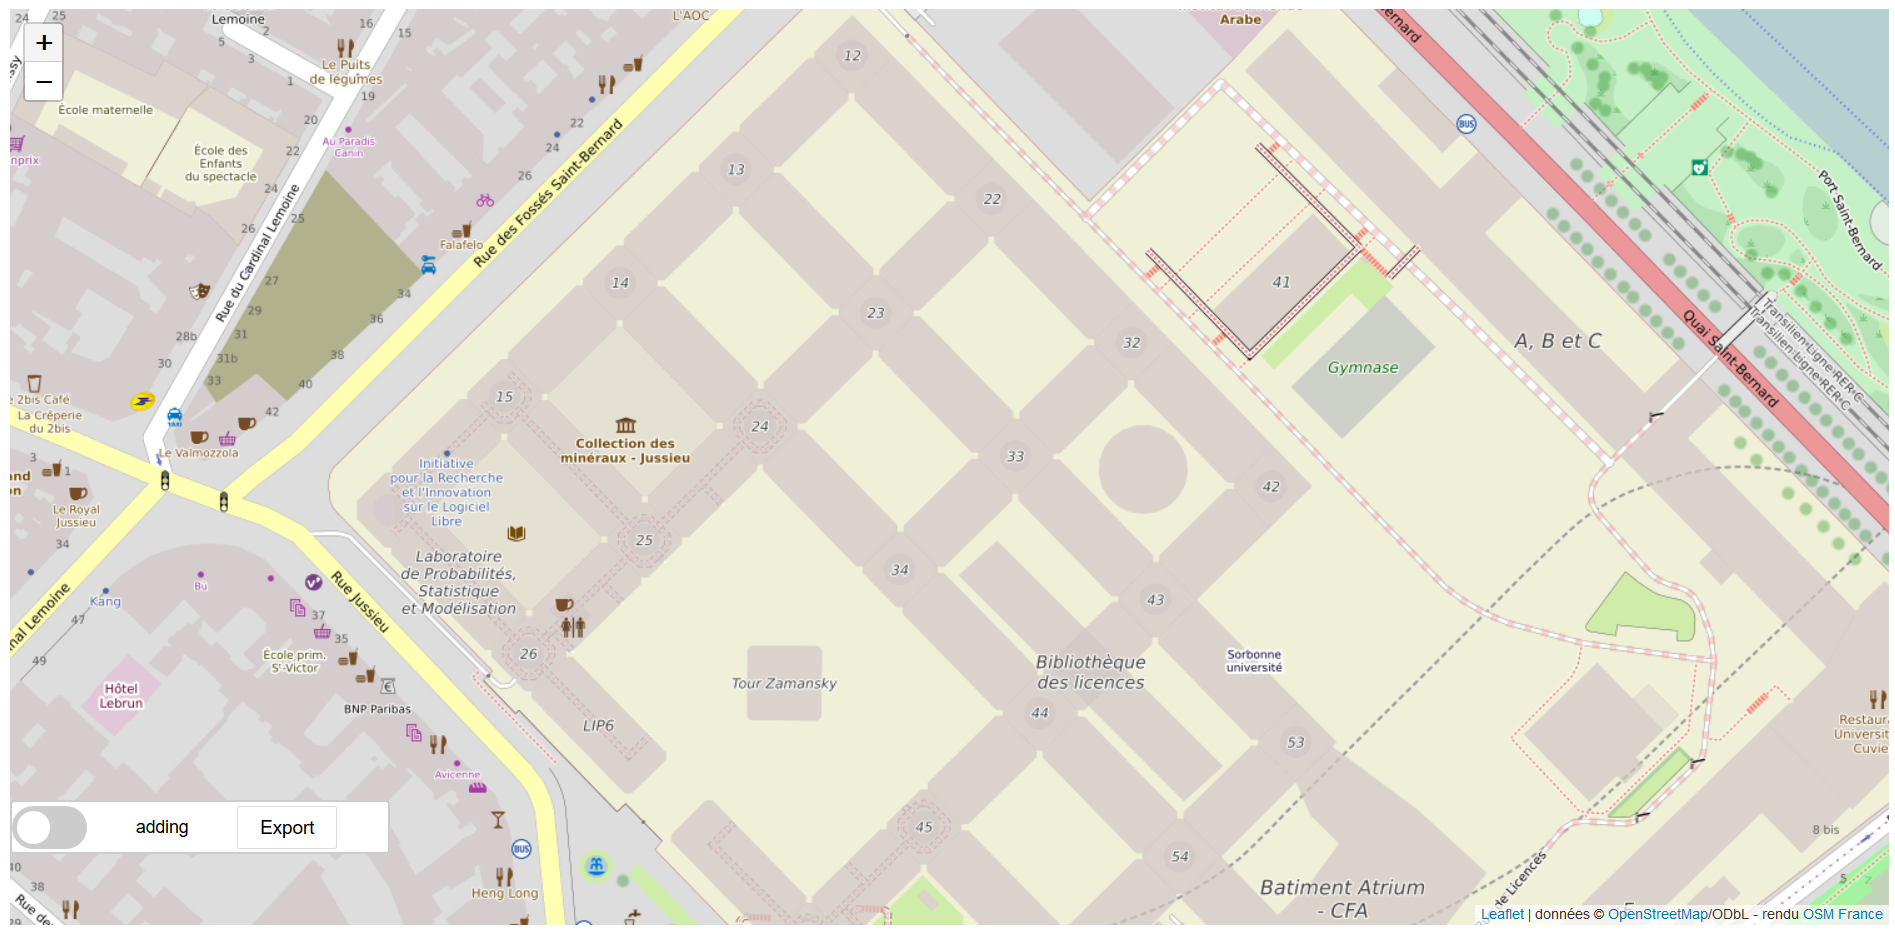
\includegraphics[scale=0.42]{capt1.PNG}\\
 La carte est interactive et on peut la déplacer avec la souris.
  Les boutons situés en haut à gauche permettent de zoomer et dézoomer sur la carte.\\
 Le cadre situé en bas à gauche contient un switch (interrupteur) et un bouton : le switch permet de changer le mode d'interaction, et le bouton permet de finaliser le plan de vol en l'exportant dans un fichier.
 Il existe deux modes d'interraction :  le mode d'ajout et le mode de suppression. Le mode dans lequel on se situe est indiqué à coté du switch ("adding" / "removing").\\
  En cliquant sur la carte, un marqueur est placé à l'endroit du clic. Chaque marqueur représente un point de passage du drone dans son itinéraire de vol. Les marqueurs peuvent être déplacés à la souris (drag and drop). Lors du survol de la souris sur un marqueur, une bulle indique son numéro d'ordre (0 pour le point de départ).
  \begin{itemize}
 \item En mode d'ajout, en cliquant sur un marqueur, on peut spécifier dans une boite de dialogue l'altitude à laquelle doit se situer le drone à ce point lors du vol.
 \item En mode de suppression, en cliquant sur un marqueur, on supprime ce dernier. Les marqueurs sont alors automatiquement remis dans le bon ordre et le trajet est retracé.
 \end{itemize}
    \medbreak
   
   \item On place des marqueurs en cliquant aux endroits voulus sur la carte. Au survol d'un marqueur, la bulle comportant son numéro d'ordre apparait :\\
 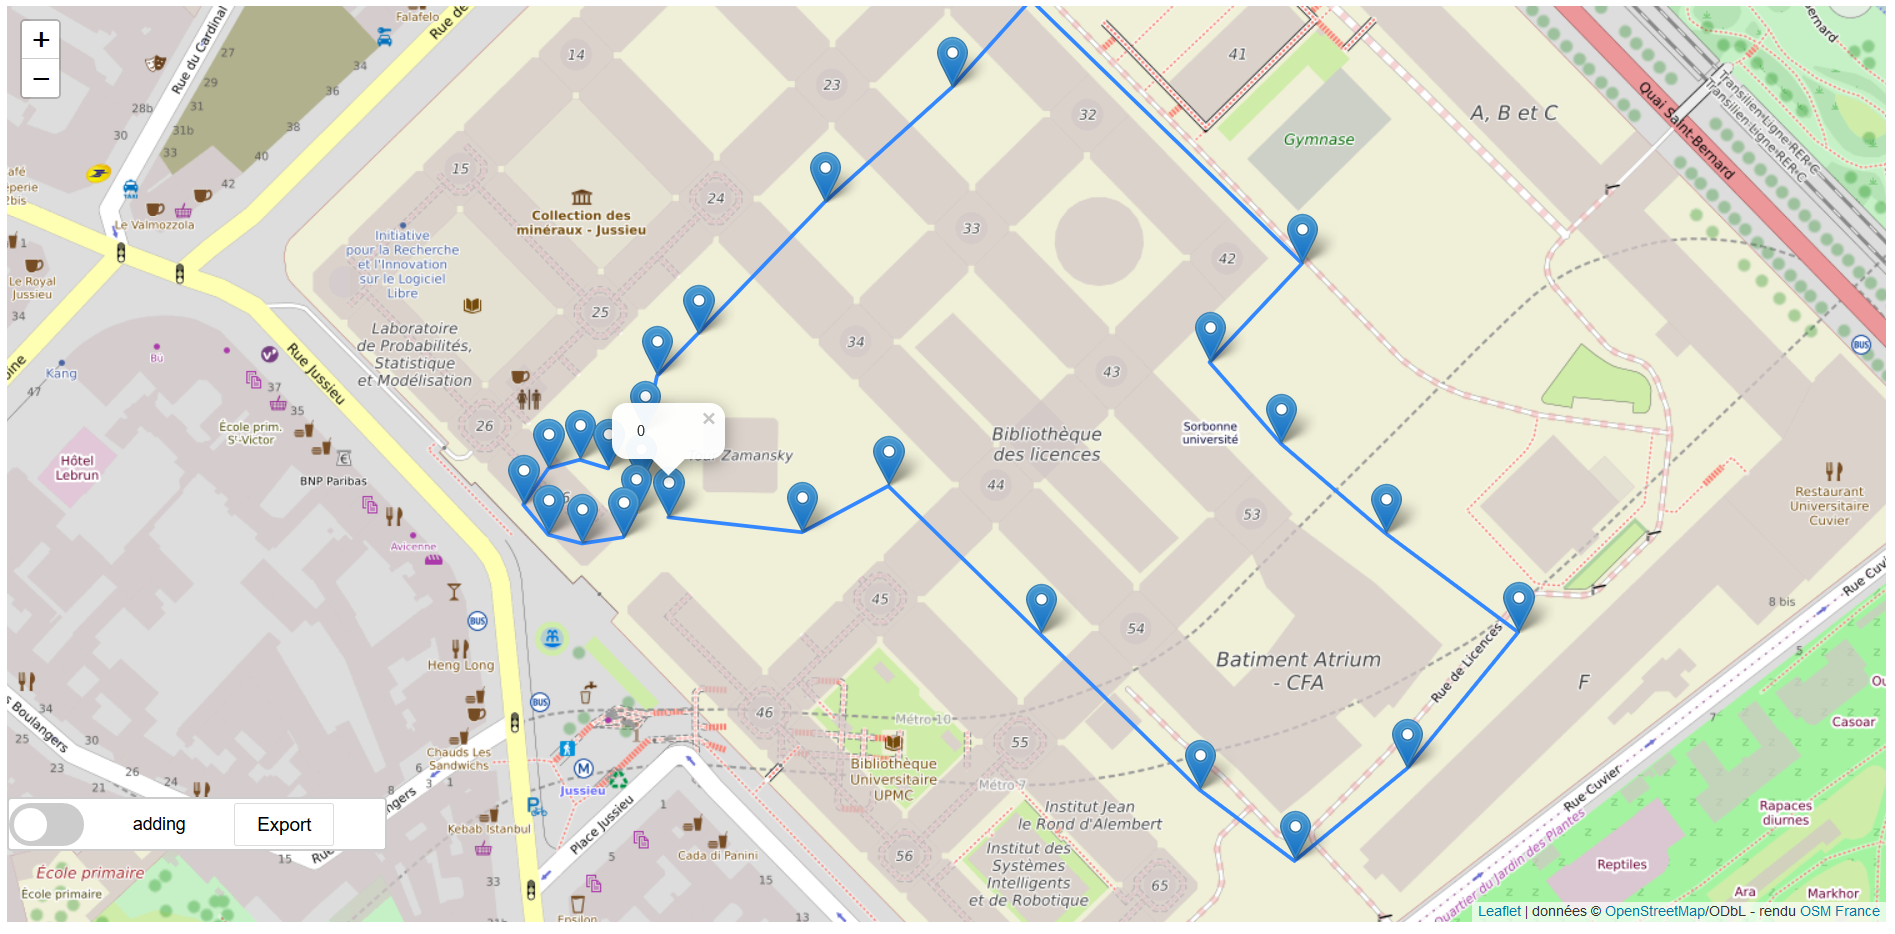
\includegraphics[scale=0.42]{capt3.PNG}
  \item On souhaite retirer des marqueurs, on active le mode de suppression en cliquant sur le switch et on clique ensuite sur les marqueurs à supprimer. L'ordre des marqueurs et le tracé du trajet d'adaptent :\\
 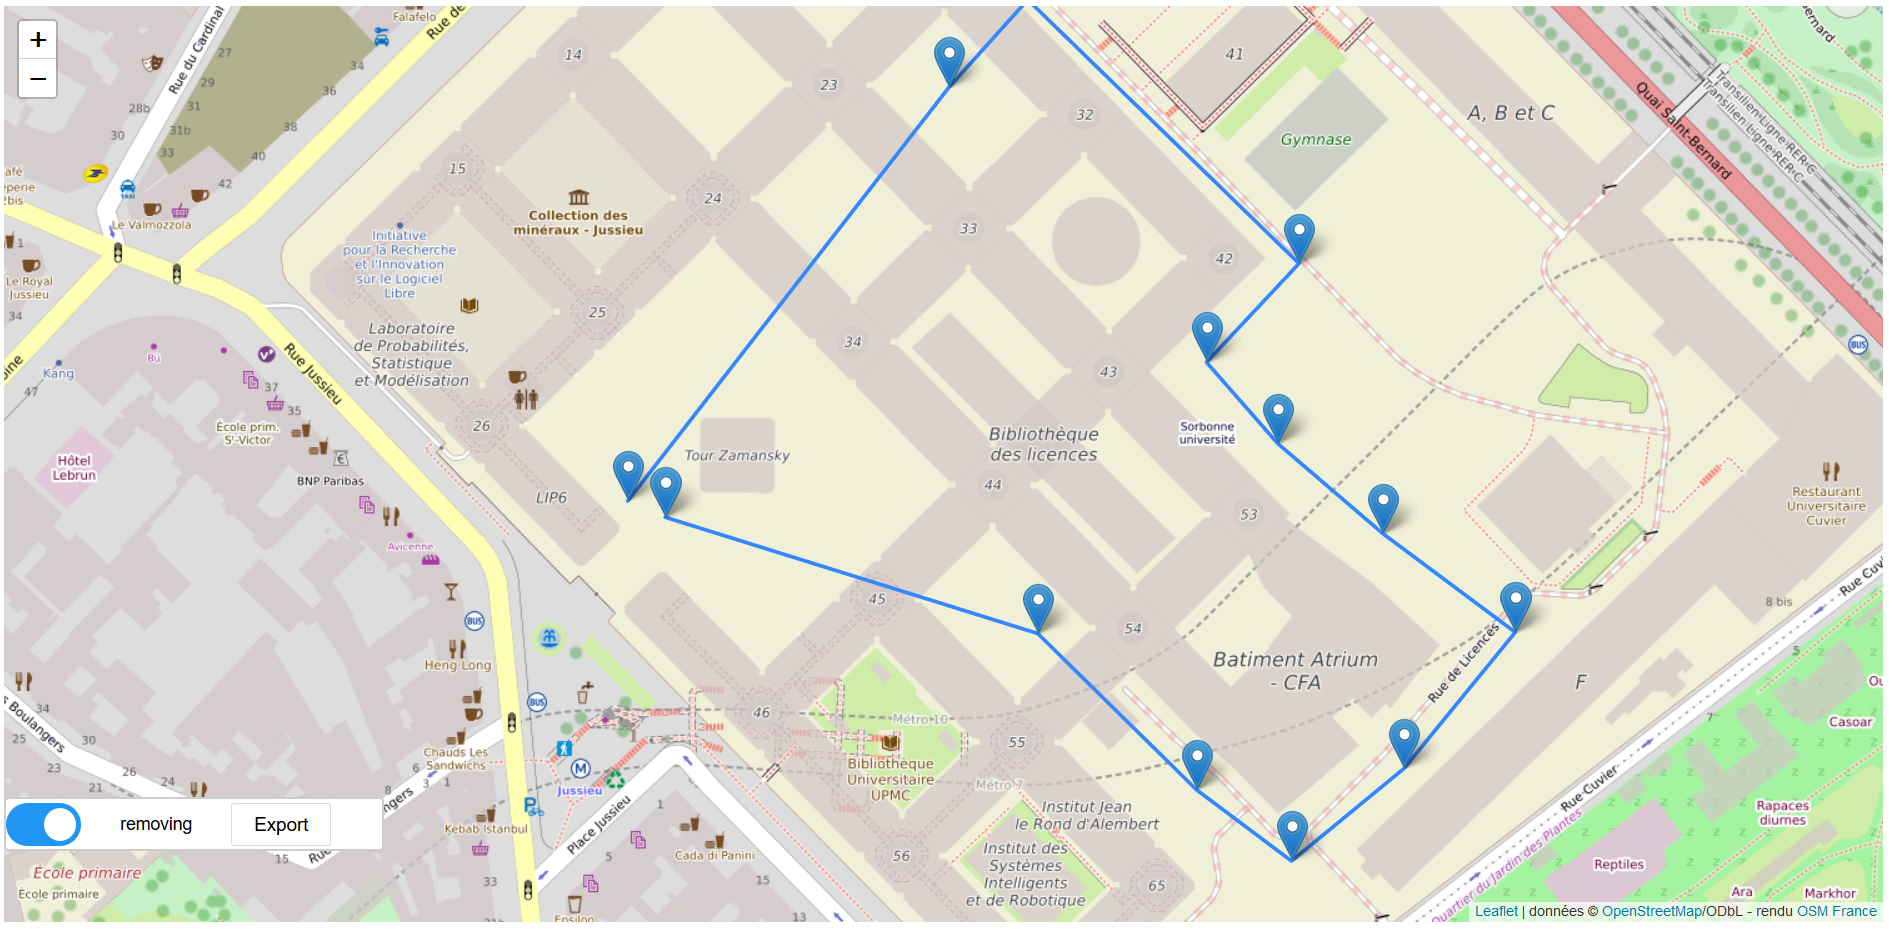
\includegraphics[scale=0.42]{capt5.PNG}
  \item On clique sur un marqueur pour spécifier l'altitude voulue à ce point :\\
 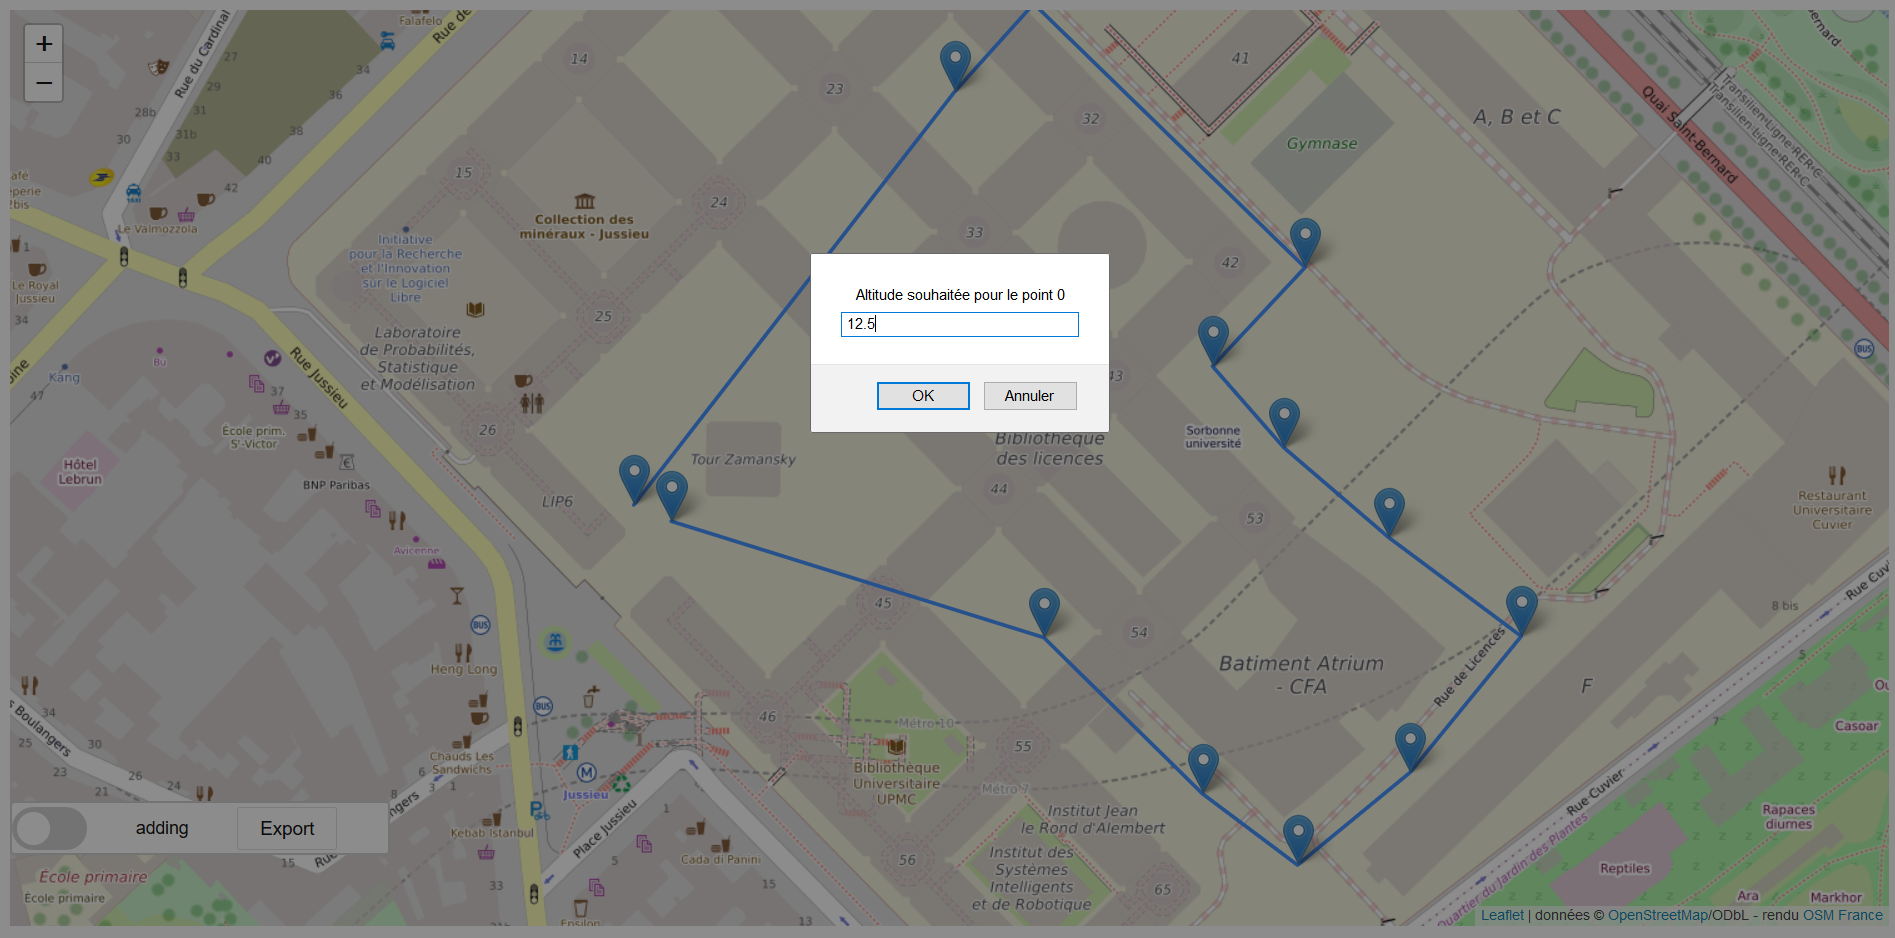
\includegraphics[scale=0.42]{capt6.PNG}
 \item On peut déplacer les marqueurs avec un cliquer-glisser (drag and drop) sur ces derniers :\\
 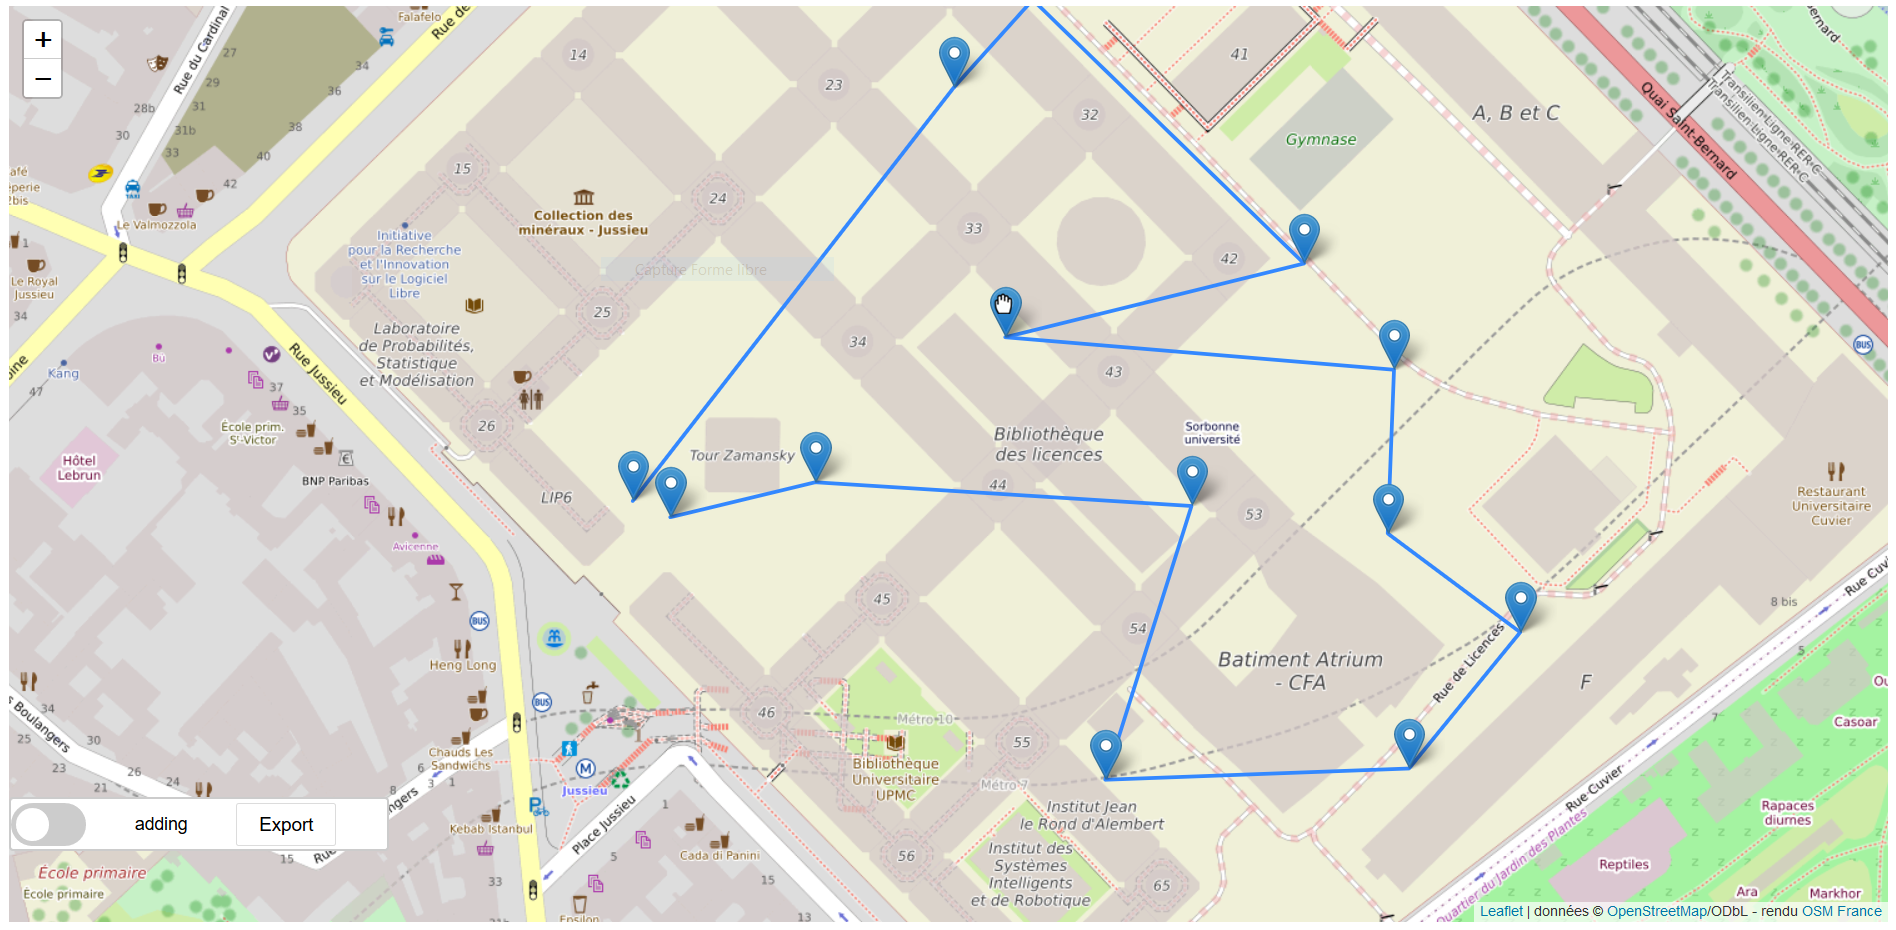
\includegraphics[scale=0.42]{capt7.PNG}
  \item Une fois le plan de vol terminé, on clique sur le bouton pour obtenir le fichier correspondant au trajet défini :\\
 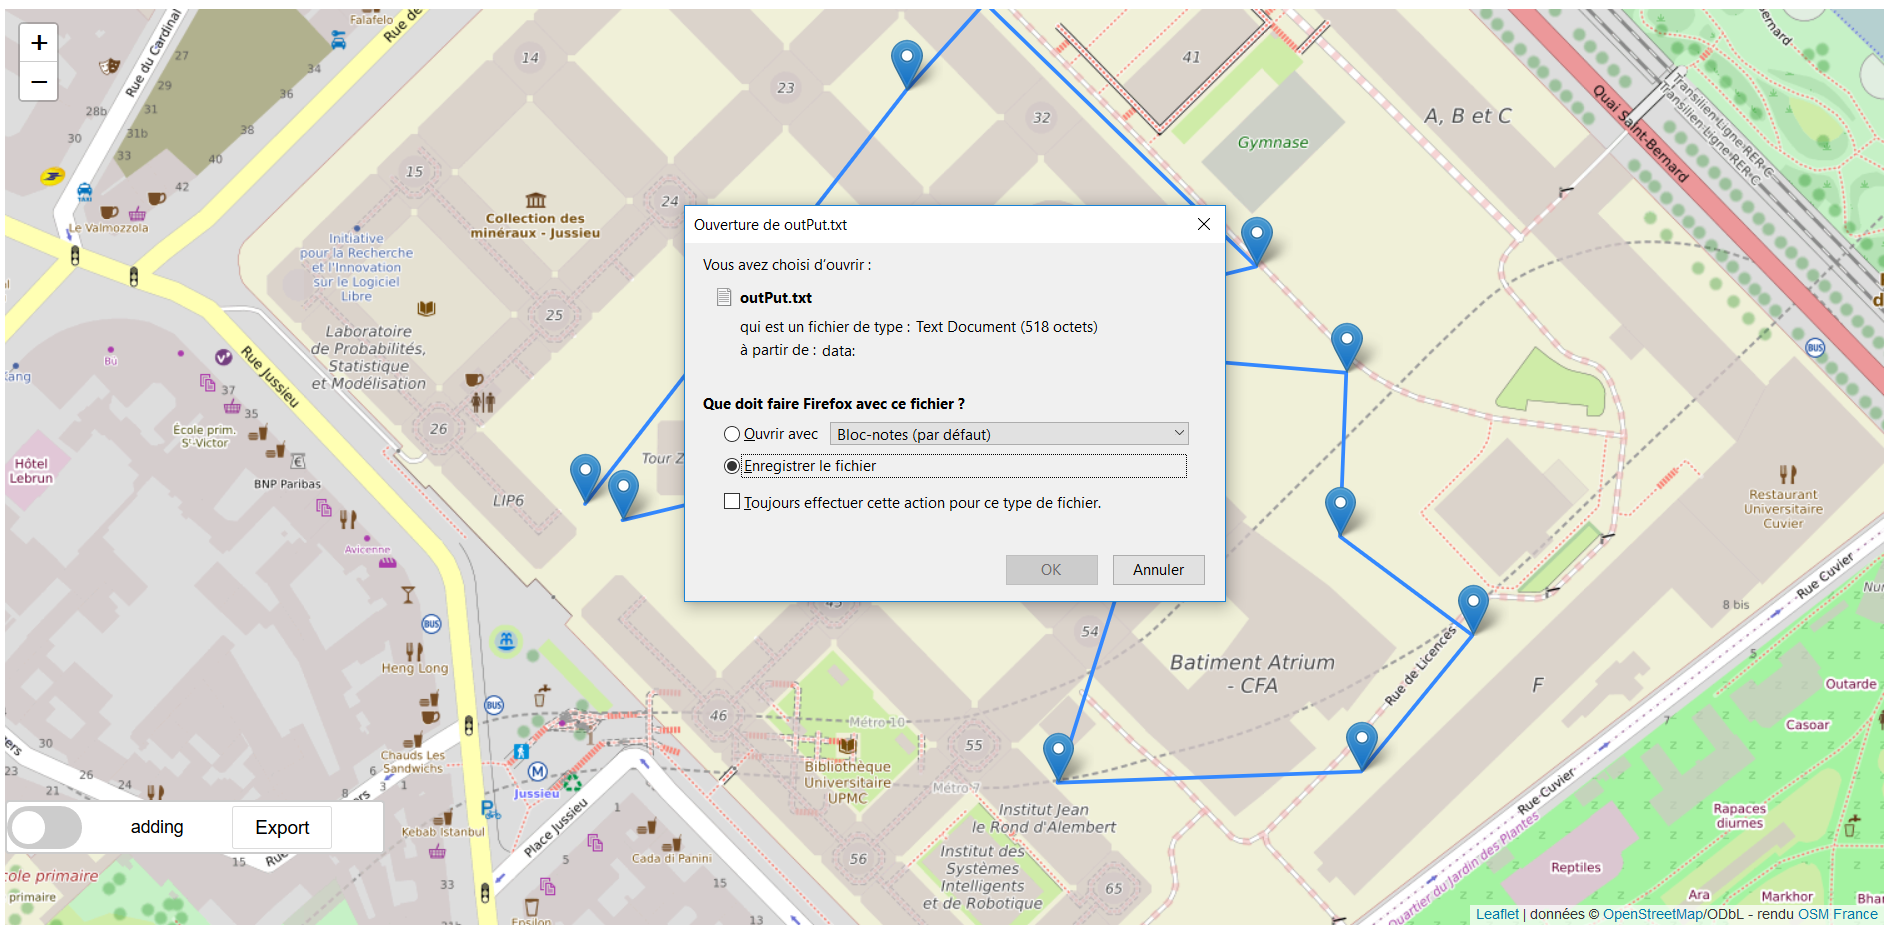
\includegraphics[scale=0.42]{capt8.PNG}

 \end{enumerate}

\end{document}
